\documentclass{beamer}\usepackage[]{graphicx}\usepackage[]{color}
%% maxwidth is the original width if it is less than linewidth
%% otherwise use linewidth (to make sure the graphics do not exceed the margin)
\makeatletter
\def\maxwidth{ %
  \ifdim\Gin@nat@width>\linewidth
    \linewidth
  \else
    \Gin@nat@width
  \fi
}
\makeatother

\definecolor{fgcolor}{rgb}{0.345, 0.345, 0.345}
\newcommand{\hlnum}[1]{\textcolor[rgb]{0.686,0.059,0.569}{#1}}%
\newcommand{\hlstr}[1]{\textcolor[rgb]{0.192,0.494,0.8}{#1}}%
\newcommand{\hlcom}[1]{\textcolor[rgb]{0.678,0.584,0.686}{\textit{#1}}}%
\newcommand{\hlopt}[1]{\textcolor[rgb]{0,0,0}{#1}}%
\newcommand{\hlstd}[1]{\textcolor[rgb]{0.345,0.345,0.345}{#1}}%
\newcommand{\hlkwa}[1]{\textcolor[rgb]{0.161,0.373,0.58}{\textbf{#1}}}%
\newcommand{\hlkwb}[1]{\textcolor[rgb]{0.69,0.353,0.396}{#1}}%
\newcommand{\hlkwc}[1]{\textcolor[rgb]{0.333,0.667,0.333}{#1}}%
\newcommand{\hlkwd}[1]{\textcolor[rgb]{0.737,0.353,0.396}{\textbf{#1}}}%

\usepackage{framed}
\makeatletter
\newenvironment{kframe}{%
 \def\at@end@of@kframe{}%
 \ifinner\ifhmode%
  \def\at@end@of@kframe{\end{minipage}}%
  \begin{minipage}{\columnwidth}%
 \fi\fi%
 \def\FrameCommand##1{\hskip\@totalleftmargin \hskip-\fboxsep
 \colorbox{shadecolor}{##1}\hskip-\fboxsep
     % There is no \\@totalrightmargin, so:
     \hskip-\linewidth \hskip-\@totalleftmargin \hskip\columnwidth}%
 \MakeFramed {\advance\hsize-\width
   \@totalleftmargin\z@ \linewidth\hsize
   \@setminipage}}%
 {\par\unskip\endMakeFramed%
 \at@end@of@kframe}
\makeatother

\definecolor{shadecolor}{rgb}{.97, .97, .97}
\definecolor{messagecolor}{rgb}{0, 0, 0}
\definecolor{warningcolor}{rgb}{1, 0, 1}
\definecolor{errorcolor}{rgb}{1, 0, 0}
\newenvironment{knitrout}{}{} % an empty environment to be redefined in TeX

\usepackage{alltt}

%%%%%%%%%%%%%%%%%%%%%%%%%%%%%%%%%%%
%%% Beamer option
%%%%%%%%%%%%%%%%%%%%%%%%%%%%%%%%%%%
\usetheme{Madrid}
\usecolortheme{beaver}
\beamertemplatenavigationsymbolsempty
\setbeamertemplate{itemize item}[triangle]
\setbeamercolor{itemize item}{fg=red}
%%%%%%%%%%%%%%%%%%%%%%%%%%%%%%%%%%%
\setbeamertemplate{footline}{}
%%%%%%%%%%%%%%%%%%%%%%%%%%%%%%%%%%%
\usepackage{lmodern}
\usepackage[english]{babel}
\usepackage{natbib}


%%%%%%%%%%%%%%%%%%%%%%%%%%%%%%%%%%%
%% Hyperlinks
\usepackage{hyperref}
\hypersetup{colorlinks=true, urlcolor=blue}



%%%%%%%%%%%%%%%%%%%%%%%%%%%%%%%%%%%
%% Maths
\usepackage{amsmath,amsthm,amssymb,amsfonts}
\newcommand{\E}{\mathbb{E}}
\newcommand{\Var}{\mathbb{V}ar}

%%%%%%%%%%%%%%%%%%%%%%%%%%%%%%%%%%%
%% Tables
\usepackage{floatrow} %centre automatic les figures
\floatsetup[table]{capposition=top}
\usepackage{multirow}
\usepackage[toc,page]{appendix}

%%%%%%%%%%%%%%%%%%%%%%%%%%%%%%%%%%%
%% Figs
\usepackage{graphicx}
\usepackage{caption}
%\usepackage{subcaption}
\graphicspath{{./figure/}}
%%%%%%%%%%%%%%%%%%%%%%%%%%%%%%%%%%%
%% Verbatim code
%\usepackage{alltt}

%%%%%%%%%%%%%%%%%%%%%%%%%%%%%%%%%%%
%% Title page
\title{ggplot2 Introduction}
\author{Jean-Baptiste Lecomte}


%%%%%%%%%%%%%%%%%%%%%%%%%%%%%%%%%%%
%% Start documents
%%%%%%%%%%%%%%%%%%%%%%%%%%%%%%%%%%%
\IfFileExists{upquote.sty}{\usepackage{upquote}}{}
\begin{document}


\maketitle


%%%%%%%%%%%%%%%%%%%%%%%%%%%%%%%%%%%
%% Introduction
%%%%%%%%%%%%%%%%%%%%%%%%%%%%%%%%%%%
\begin{frame}{Introduction}
  \begin{itemize}
    \item developped by Hadley Wickham (Rice University, Houston, USA)
    \item highly recommanded R packages to work with ggplot2: reshape and plyr (also developped by H. Wickham)
    \item first version called in 2007
  \end{itemize}
\end{frame}

\begin{frame}{Useful books}
  \begin{columns}
    \begin{column}{0.5\textwidth}
      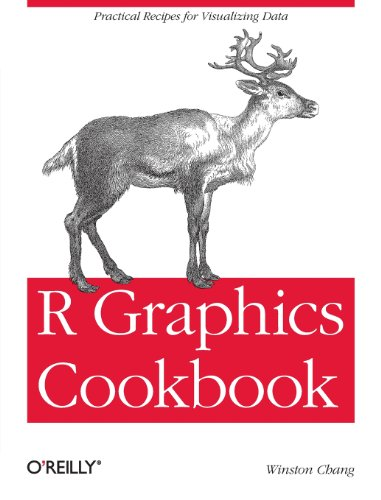
\includegraphics[scale=0.45]{rgraphicscookbook}
    \end{column}
  
    \begin{column}{0.5\textwidth}
      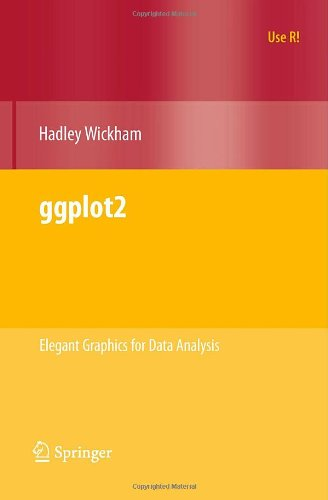
\includegraphics[scale=0.45]{ggplot2}
    \end{column}
  \end{columns}
\end{frame}

\begin{frame}{Online ressources}
    	\begin{itemize}
    	  \item ggplot2 official documentation:\\  \url{http://docs.ggplot2.org/current/}
        \item R code related to ggplot2 cookbook:\\ \url{http://www.cookbook-r.com/Graphs/}
        \item R code related to useR! ggplot2 book:\\ \url{http://ggplot2.org/book/}
  		  \item Google groups to ask questions:\\ \url{ggplot2@googlegroups.com}
        \item Github repository:\\ \url{https://github.com/yhat/ggplot/}
			\end{itemize}
\end{frame}


\begin{frame}{Introduction}
  \begin{itemize}
    \item based on new aesthetic principles
    \item based on \textit{The grammar of graphics} developed by Wilkinson in 2005
    \item efficient way to produce simple graphics with a length reduction of R code
  \end{itemize}
  
  \begin{alertblock}{Forget about R base graphics:}
     \texttt{ plot(), hist(), par(), layout(), points(), lines(),legend()}
  \end{alertblock}
\end{frame}

\begin{frame}{Principle}
ggplot2 is based on a \textbf{layer} system which can be used as objects.\\
\vspace{1cm}
Main layers
  \begin{itemize}
    \item data $\rightarrow$ raw data
    \item mapping $\rightarrow$ graphic projection
    \item geom $\rightarrow$ geometric objects (points, lines, polygons, ...)
    \item stat $\rightarrow$ statistics transformation (histogram, model)
    \item scale $\rightarrow$ aesthetics customization (color, shape, size, axes, legend)
    \item coord $\rightarrow$ coordinate system (axes, grid)
    \item facet $\rightarrow$ subdivision (lattice, trellis)
  \end{itemize}
\end{frame}

\begin{frame}{Base functions}
ggplot2 is based on two functions:
  \begin{enumerate}
		\item  \texttt{qplot()} for \textbf{q}uick \textbf{plot}
		\begin{itemize}
			\item easy and fast, but too simple in most cases
			\item \texttt{qplot(x, y, data=data)}
		\end{itemize}
    \vspace{0.5cm}
    \item \texttt{ggplot()}
      	\begin{itemize}
			\item more complex but more powerful and flexible by adding \texttt{layers}
			\item \texttt{ggplot(data=data, aes(x, y)) + layers}
		\end{itemize}
  \end{enumerate}
\end{frame}


\begin{frame}[fragile]{Getting Started}

  \begin{alertblock}{Data format}
    Always work with a \texttt{data.frame}
  \end{alertblock}
    Our data frame is based on the surveys XXXX and simulated data.
    Github repository:\\ \url{https://github.com/JBLecomte/ggplot2-Introduction.git}
\end{frame}

\begin{frame}[fragile]{Getting Started}
\begin{knitrout}\scriptsize
\definecolor{shadecolor}{rgb}{0.969, 0.969, 0.969}\color{fgcolor}\begin{kframe}
\begin{alltt}
  \hlkwd{str}\hlstd{(df_data)}
\end{alltt}
\begin{verbatim}
## 'data.frame':	1909 obs. of  18 variables:
##  $ Year            : int  2005 2005 2005 2005 2005 2005 2005 2005 2005 2005 ...
##  $ Month           : int  7 7 7 7 7 7 7 7 7 7 ...
##  $ DURATION_MINUTES: int  21 20 21 21 20 20 20 21 21 20 ...
##  $ AREA            : Factor w/ 2 levels "5AB","5CD": 1 1 1 1 1 1 1 1 1 1 ...
##  $ Avg_net_depth   : num  -0.316 -0.435 -0.442 -0.234 -0.171 ...
##  $ Avg_net_temp    : num  0.3939 0.4339 0.3004 0.1335 -0.0267 ...
##  $ Date            : Date, format: "2005-07-06" "2005-07-06" ...
##  $ Lon             : num  -128 -128 -128 -128 -128 ...
##  $ Lat             : num  51.2 51.1 51.6 51.6 51.7 ...
##  $ X               : num  572025 570307 553665 551917 546338 ...
##  $ Y               : num  5668122 5665874 5717947 5719597 5723992 ...
##  $ X_km            : num  572 570 554 552 546 ...
##  $ Y_km            : num  5668 5666 5718 5720 5724 ...
##  $ Pres            : num  1 1 1 1 1 1 1 0 0 1 ...
##  $ Year_fac        : Factor w/ 5 levels "2005","2007",..: 1 1 1 1 1 1 1 1 1 1 ...
##  $ AREA_num        : num  1 1 1 1 1 1 1 1 1 1 ...
##  $ nFish           : int  3 2 1 2 4 2 0 1 2 5 ...
##  $ Biomass         : num  7.69 5.25 2.45 4.61 10.7 ...
\end{verbatim}
\end{kframe}
\end{knitrout}
\end{frame}

%%%%%%%%%%%%%%%%%%%%%%%%%%%%%%%%%%%
%% Example
%%%%%%%%%%%%%%%%%%%%%%%%%%%%%%%%%%%

\begin{frame}[fragile]{Scatter plot: Depth and Biomass}
\begin{knitrout}\footnotesize
\definecolor{shadecolor}{rgb}{0.969, 0.969, 0.969}\color{fgcolor}\begin{kframe}
\begin{alltt}
  \hlstd{scatter_plot} \hlkwb{<-} \hlkwd{ggplot}\hlstd{(}\hlkwc{data}\hlstd{=df_data,} \hlkwd{aes}\hlstd{(}\hlkwc{x}\hlstd{=Avg_net_depth,} \hlkwc{y}\hlstd{=Biomass))} \hlopt{+}
                \hlkwd{geom_point}\hlstd{()}
  \hlkwd{print}\hlstd{(scatter_plot)}
\end{alltt}
\end{kframe}

{\centering 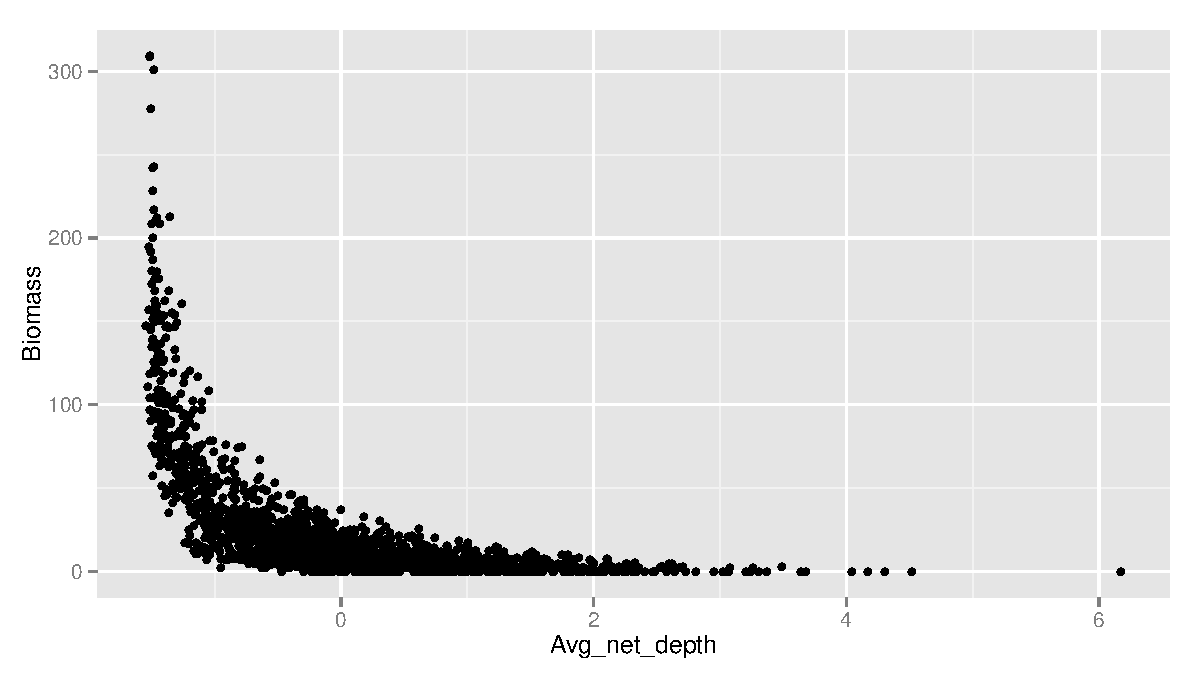
\includegraphics[width=.9\linewidth]{figure/scatter_plot_base-1} 

}



\end{knitrout}
\end{frame}

\begin{frame}[fragile]{Scatter plot with color: Depth and Biomass}
\begin{knitrout}\footnotesize
\definecolor{shadecolor}{rgb}{0.969, 0.969, 0.969}\color{fgcolor}\begin{kframe}
\begin{alltt}
  \hlstd{scatter_plot_color} \hlkwb{<-} \hlkwd{ggplot}\hlstd{(df_data,} \hlkwd{aes}\hlstd{(}\hlkwc{x}\hlstd{=Avg_net_depth,} \hlkwc{y}\hlstd{=Biomass,}
                                         \hlkwc{color}\hlstd{=AREA))} \hlopt{+}
  \hlkwd{geom_point}\hlstd{()}
  \hlkwd{print}\hlstd{(scatter_plot_color)}
\end{alltt}
\end{kframe}

{\centering 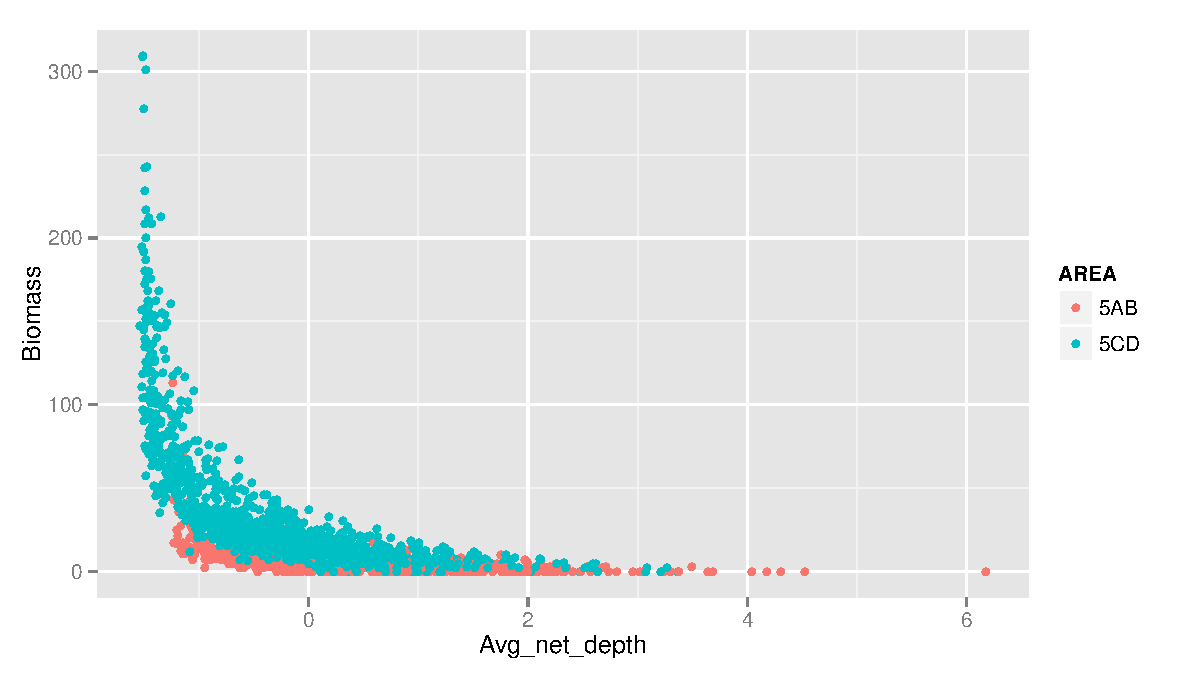
\includegraphics[width=.9\linewidth]{figure/scatter_plot_color-1} 

}



\end{knitrout}
\end{frame}


\begin{frame}[fragile]{Scatter plot with shape: Depth and Biomass}
\begin{knitrout}\footnotesize
\definecolor{shadecolor}{rgb}{0.969, 0.969, 0.969}\color{fgcolor}\begin{kframe}
\begin{alltt}
  \hlstd{scatter_plot_shape} \hlkwb{<-} \hlkwd{ggplot}\hlstd{(df_data,} \hlkwd{aes}\hlstd{(}\hlkwc{x}\hlstd{=Avg_net_depth,} \hlkwc{y}\hlstd{=Biomass,}
                                         \hlkwc{color}\hlstd{=AREA,} \hlkwc{shape}\hlstd{=Year_fac))} \hlopt{+}
  \hlkwd{geom_point}\hlstd{()}
  \hlkwd{print}\hlstd{(scatter_plot_shape)}
\end{alltt}
\end{kframe}

{\centering 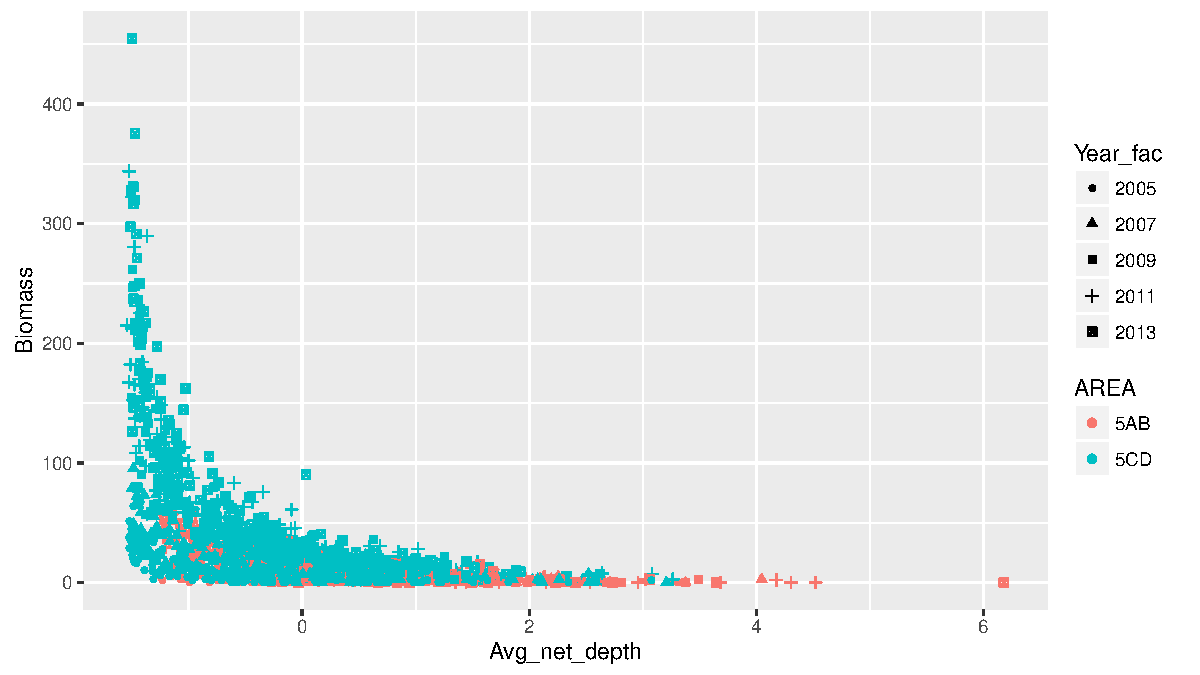
\includegraphics[width=.9\linewidth]{figure/scatter_plot_shape-1} 

}



\end{knitrout}
\end{frame}

\begin{frame}[fragile]{Scatter plot with continuous color: Depth and Biomass}
\begin{knitrout}\footnotesize
\definecolor{shadecolor}{rgb}{0.969, 0.969, 0.969}\color{fgcolor}\begin{kframe}
\begin{alltt}
  \hlstd{scatter_plot_color_cont} \hlkwb{<-} \hlkwd{ggplot}\hlstd{(df_data,} \hlkwd{aes}\hlstd{(}\hlkwc{x}\hlstd{=Avg_net_depth,} \hlkwc{y}\hlstd{=Biomass,}
                                         \hlkwc{color}\hlstd{=Avg_net_temp))} \hlopt{+}
  \hlkwd{geom_point}\hlstd{()}
  \hlkwd{print}\hlstd{(scatter_plot_color_cont)}
\end{alltt}
\end{kframe}

{\centering 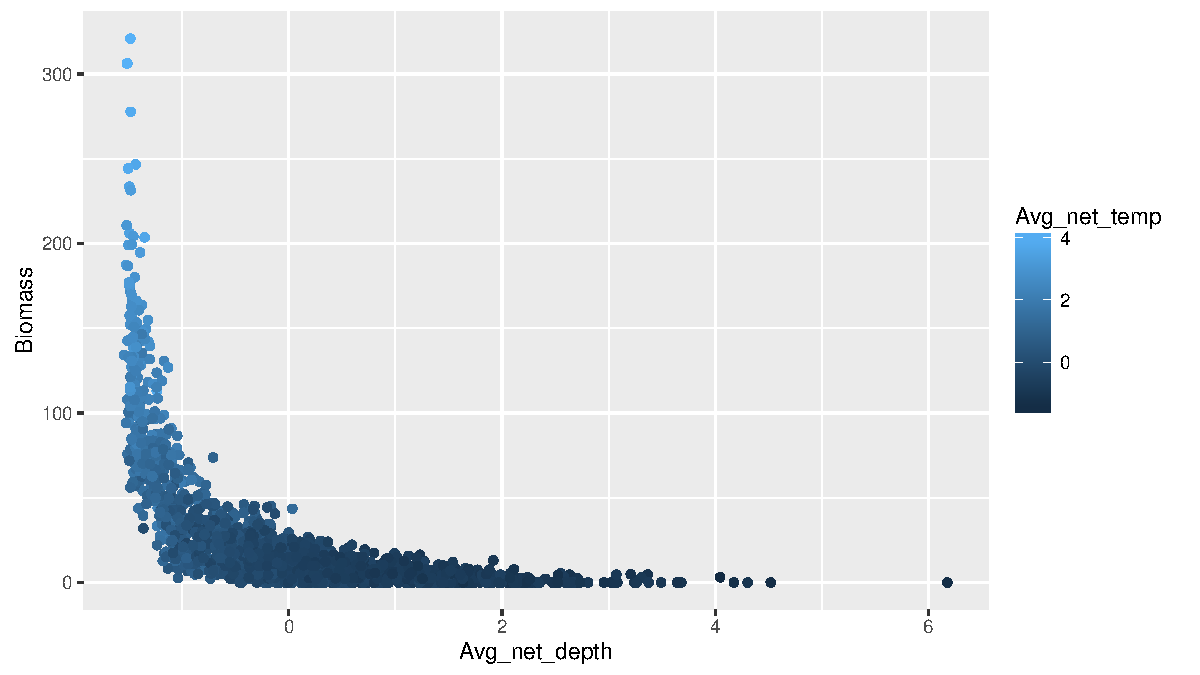
\includegraphics[width=.9\linewidth]{figure/scatter_plot_color_cont-1} 

}



\end{knitrout}
\end{frame}


\begin{frame}[fragile]{Scatter plot with size: Depth and Biomass}
\begin{knitrout}\footnotesize
\definecolor{shadecolor}{rgb}{0.969, 0.969, 0.969}\color{fgcolor}\begin{kframe}
\begin{alltt}
  \hlstd{scatter_plot_area} \hlkwb{<-} \hlkwd{ggplot}\hlstd{(df_data,} \hlkwd{aes}\hlstd{(}\hlkwc{x}\hlstd{=Avg_net_depth,} \hlkwc{y}\hlstd{=Biomass,}
                                         \hlkwc{size}\hlstd{=Avg_net_temp))} \hlopt{+}
  \hlkwd{geom_point}\hlstd{()}
  \hlkwd{print}\hlstd{(scatter_plot_area)}
\end{alltt}
\end{kframe}

{\centering 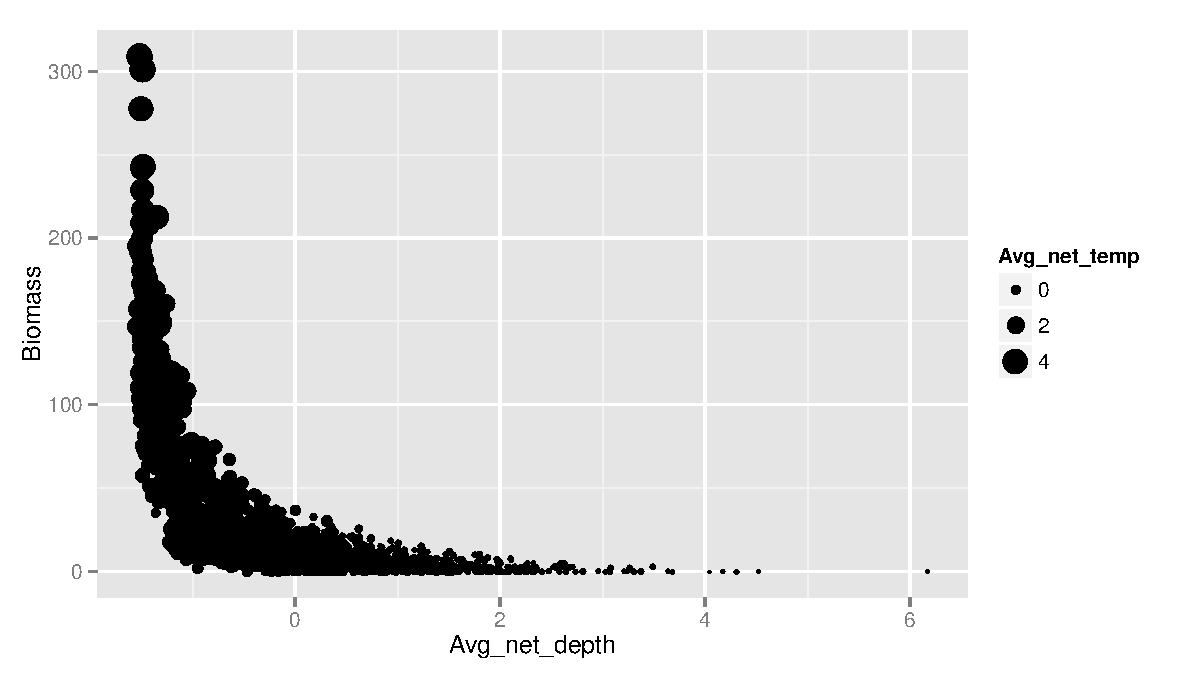
\includegraphics[width=.9\linewidth]{figure/scatter_plot_color_size-1} 

}



\end{knitrout}
\end{frame}

\begin{frame}[fragile]{Improvement of a plot}
\begin{knitrout}\footnotesize
\definecolor{shadecolor}{rgb}{0.969, 0.969, 0.969}\color{fgcolor}\begin{kframe}
\begin{alltt}
  \hlkwd{print}\hlstd{(scatter_plot_shape)}
\end{alltt}
\end{kframe}

{\centering 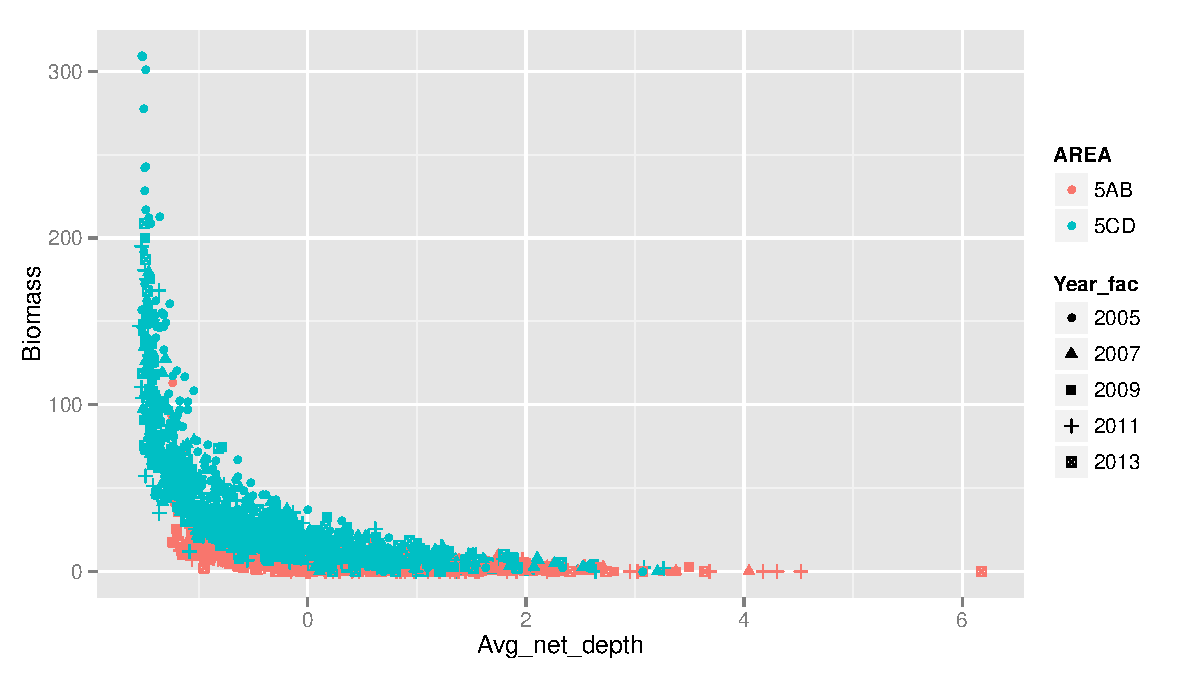
\includegraphics[width=.9\linewidth]{figure/scatter_plot_shape2-1} 

}



\end{knitrout}
\end{frame}

\begin{frame}[fragile]{Improvement of a plot: axes names}
\begin{knitrout}\footnotesize
\definecolor{shadecolor}{rgb}{0.969, 0.969, 0.969}\color{fgcolor}\begin{kframe}
\begin{alltt}
  \hlstd{scatter_plot_shape_imp1} \hlkwb{<-} \hlstd{scatter_plot_shape} \hlopt{+}
  \hlkwd{xlab}\hlstd{(}\hlstr{'Average net depth (in m)'}\hlstd{)} \hlopt{+} \hlkwd{ylab}\hlstd{(}\hlstr{'Biomass (in kg)'}\hlstd{)}

  \hlkwd{print}\hlstd{(scatter_plot_shape_imp1)}
\end{alltt}
\end{kframe}

{\centering 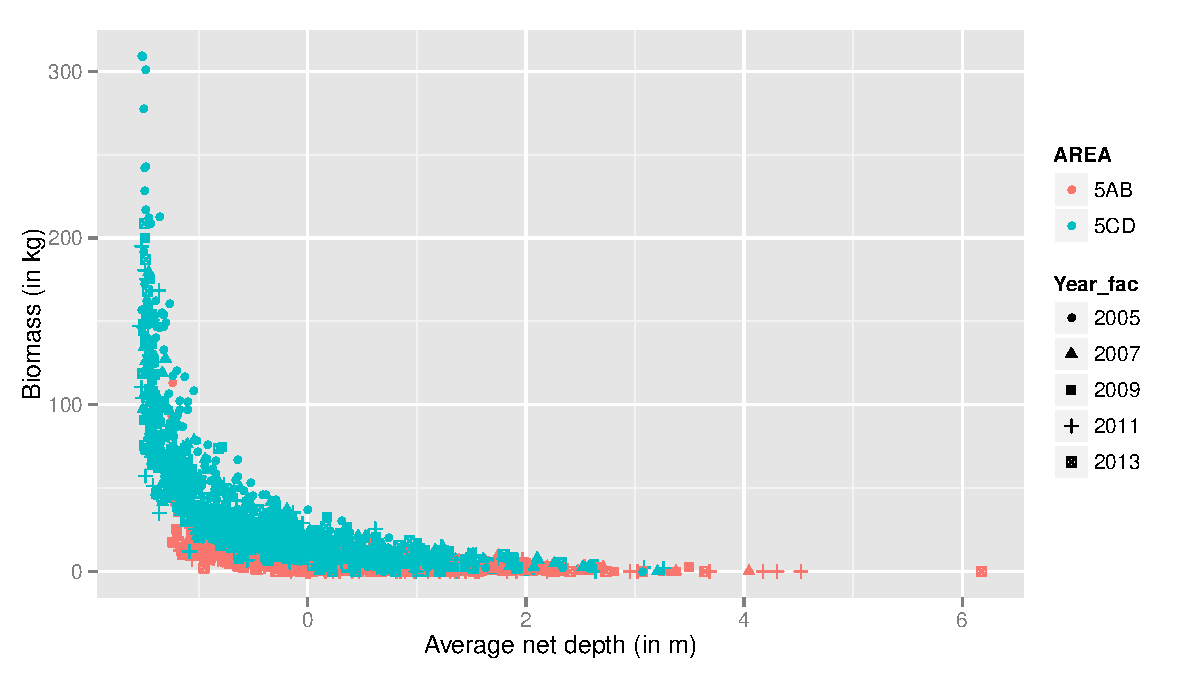
\includegraphics[width=.9\linewidth]{figure/scatter_plot_shape_imp1-1} 

}



\end{knitrout}
\end{frame}

\begin{frame}[fragile]{Improvement of a plot: legend titles}
\begin{knitrout}\footnotesize
\definecolor{shadecolor}{rgb}{0.969, 0.969, 0.969}\color{fgcolor}\begin{kframe}
\begin{alltt}
  \hlstd{scatter_plot_shape_imp2} \hlkwb{<-} \hlstd{scatter_plot_shape_imp1} \hlopt{+}
  \hlkwd{scale_shape_discrete}\hlstd{(}\hlkwc{name}\hlstd{=}\hlstr{"Years"}\hlstd{)} \hlopt{+}
  \hlkwd{scale_color_discrete}\hlstd{(}\hlkwc{name}\hlstd{=}\hlstr{"Area"}\hlstd{)}

  \hlkwd{print}\hlstd{(scatter_plot_shape_imp2)}
\end{alltt}
\end{kframe}

{\centering 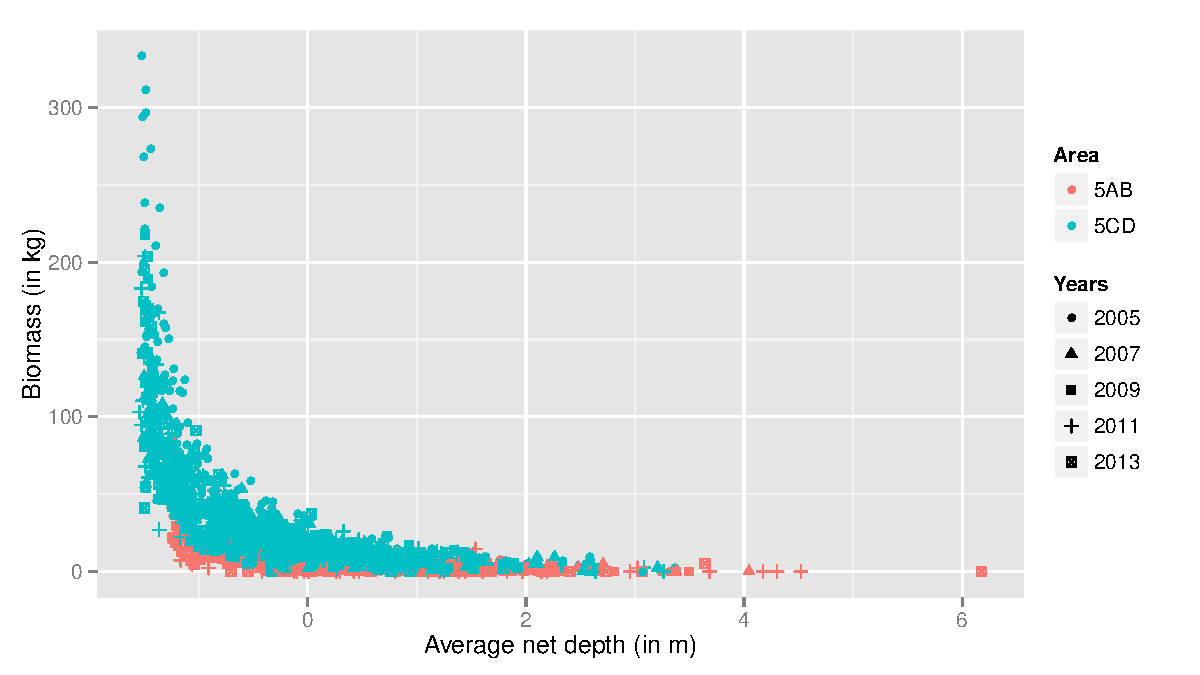
\includegraphics[width=.9\linewidth]{figure/scatter_plot_shape_imp2-1} 

}



\end{knitrout}
\end{frame}


\begin{frame}[fragile]{Improvement of a plot: plot title}
\begin{knitrout}\footnotesize
\definecolor{shadecolor}{rgb}{0.969, 0.969, 0.969}\color{fgcolor}\begin{kframe}
\begin{alltt}
  \hlstd{scatter_plot_shape_imp3} \hlkwb{<-} \hlstd{scatter_plot_shape_imp2} \hlopt{+}
   \hlkwd{ggtitle}\hlstd{(}\hlstr{"Biomass of species X and average net depth"}\hlstd{)}

  \hlkwd{print}\hlstd{(scatter_plot_shape_imp3)}
\end{alltt}
\end{kframe}

{\centering 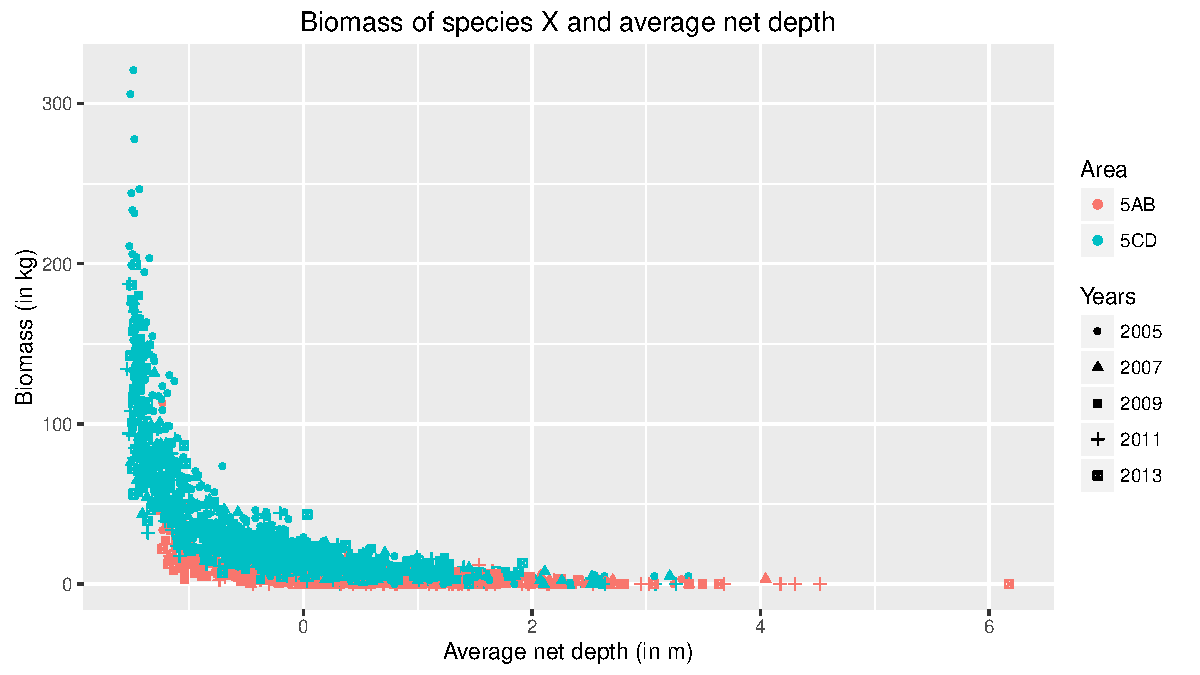
\includegraphics[width=.9\linewidth]{figure/scatter_plot_shape_imp3-1} 

}



\end{knitrout}
\end{frame}

\end{document}
